\documentclass{article}
\usepackage[utf8]{inputenc}
\usepackage[T1]{fontenc}
\usepackage{lipsum}
\usepackage{graphicx}
\usepackage{amsmath}
\usepackage[margin=1in]{geometry}
\usepackage{titlesec}
\usepackage{graphicx}
\usepackage{floatflt,epsfig}
\usepackage[utf8]{inputenc}
\usepackage[T1]{fontenc}
\usepackage{lipsum}
\usepackage{graphicx}
\usepackage{amsmath}
\usepackage[margin=1in]{geometry}
\usepackage{titlesec}
\usepackage{listings}
\usepackage{xcolor}
\usepackage{hyperref}
\usepackage{subfigure}
\usepackage{graphicx}

\hypersetup{
    pdfborder = {0 0 0},
}

\lstdefinelanguage{Java}{
  keywords={abstract,assert,boolean,break,byte,case,catch,char,class,const,continue,default,do,double,else,enum,extends,false,final,finally,float,for,goto,if,implements,import,instanceof,int,interface,long,native,new,null,package,private,protected,public,return,short,static,strictfp,super,switch,synchronized,this,throw,throws,transient,true,try,void,volatile,while},
  morekeywords={[2]System,out},
  morecomment=[l]{//},
  morecomment=[s]{/*}{*/},
  morestring=[b]",
  basicstyle=\small\ttfamily,
  keywordstyle=\color{blue}\bfseries,
  keywordstyle={[2]\color{orange}\bfseries},
  commentstyle=\color{green!70!black},
  stringstyle=\color{red},
  showstringspaces=false,
  tabsize=2,
  breaklines=true,
  breakatwhitespace=true,
  frame=single,
  captionpos=b
}

\titleformat{\section}
{\LARGE\bfseries}{\thesection}{1em}{}

\titleformat{\subsection}
{\Large\bfseries}{\thesection}{1em}{}

\begin{document}

\pagestyle{empty}

\begin{titlepage}
    \begin{center}
        {{\Large{\textsc{Alma Mater Studiorum - Università di Bologna}}}}
        \rule[0.1cm]{\textwidth}{0.1px}
        \rule[0.5cm]{\textwidth}{0.6px}\\
        {\large{SCUOLA DI SCIENZE \\ Corso di Laurea in Informatica per il Management}}
    \end{center}

    \vspace{90px}

    \begin{center}
        \LARGE Personal Physical Tracker
    \end{center}

    \vspace{100px}
    \par
    \noindent
    \hfill
    \begin{minipage}[t]{0.4\textwidth}\raggedleft
    {\fontsize{12}{13}{}\
    \fontsize{12}{13}{\\ Canghiari Matteo \\ Matricola 1032059 \\ matteo.canghiari@studio.unibo.it}}

    {\fontsize{12}{13}{}\
    \fontsize{12}{13}{\\ Rocca Claudio \\ Matricola 1032059 \\ claudio.rocca@studio.unibo.it}}
    \end{minipage}

    \vspace*{140px}

    \begin{center}
        \large{Laboratorio di Applicazioni Mobili}\\
        \large{Anno Accademico 2023/2024}
    \end{center}
\end{titlepage}

\newpage
\subsection*{Introduzione}
\large

\textbf{Personal Physical Tracker}, è un'applicazione nativa Android che permette di registrare le attività compiute durante la giornata, contraddistinte in \textbf{camminata}, \textbf{spostamenti in macchina} e \textbf{attività sedentarie}.
L'applicazione si avvale di differenti funzionalità, dalla registrazione delle attività compiute sino alla visualizzazione dei dati di altri utenti presenti sull'applicativo. Tutte le funzionalità presenti saranno successivamente approfondite nella sezione \textbf{Feature}, tuttavia è possibile anticipare ciò che contraddistingue il sistema software ideato. \vspace*{7pt}\\
Ad un primo avvio l'utente visualizzerà una finestra in grado di sovrapporre un frammento di \textit{Login} e di \textit{Sign In}, caratterizzata dai canonici controlli relativi all'\textit{accesso} e \textit{registrazione} dell'applicazione. Proseguendo, verrà mostrato il fulcro dell'app, composto da una \textit{Navigation Bottom Bar}, garantendo in questo modo l'accesso diretto alle funzionalità sviluppate. \\
In questa sezione l'utente avrà la possibilità di \textbf{registrare} nuove attività, \textbf{visualizzare} il proprio storico, osservare le proprie \textbf{aree geografiche di interesse}, visualizzare i \textbf{grafici} relativi alle proprie attività registrate ed, infine, condividere e visualizzare le attività condivise da altri utenti nella sezione \textbf{amici}. \vspace*{7pt}\\
Descritto un breve riepilogo delle peculiarità che possiede l'applicazione, è bene soffermarsi sulle scelte implementative effettuate, in maniera tale da esprimere al meglio il ragionamento dedotto durante lo sviluppo; anche in questa circostanza verranno solamente anticipate alcune tematiche. \vspace*{7pt}\\
Per il versionamento del codice è stato utilizzato \textbf{Git}, con repository accessibile su \textbf{GitHub}, mentre per lo sviluppo dell'applicativo è stato utilizzato il linguaggio di programmazione \textbf{Kotlin}, per la realizzazione di un'applicazione \textbf{nativa Android}. Il progetto si compone di tre punti cardine per il corretto funzionamento, suddivisi come segue:
\begin{itemize}
    \renewcommand{\labelitemi}{-}
    \item Design pattern architetturale \textbf{MVVM}, adeguato affinchè sia possibile porre un layer aggiuntivo tra il \textit{contenitore statico} di dati, coincidente con il \textbf{Model}, e la sezione \textit{attiva}, definita all'interno della \textbf{View}. In questo modo sono ovviate \textit{dipendenze funzionali}, che potrebbero possedere un effetto distruttivo sull'entità sviluppate, dove piccole modifiche potrebbero compromettere la stabilità del progetto
    \item \textbf{Room}, utilizzato per garantire la persistenza dei dati all'interno di un \textit{Database Relazionale}
    \item \textbf{Amazon S3}, utilizzato per salvare in cloud i dati degli utenti attraverso un \textit{database dump}, consentendo la condivisione dei dati salvati sul \textit{database locale} e permettendo di visualizzare i dati condivisi dagli amici
\end{itemize}

\newpage
\subsection*{Feature}
\textit{Registrazione} \vspace*{7pt}\\
All'avvio dell'app è richiesta la registrazione delle credenziali, suddivise in \textit{username} e \textit{password}. E' necessario registrarsi con un username non ancora presente, per garantire l' univocità dei dati. Una volta registrato, all'utente sarà richiesto di concedere tutti i permessi necessari per il funzionamento dell'applicazione. \\
Tra i permessi richiesti sono presenti:
\begin{itemize}
    \renewcommand{\labelitemi}{-}
    \item \textbf{Access fine location}, autorizzazione di accesso alla posizione corrente del dispositivo, necessaria per monitorare le aree geografiche varcate
    \item \textbf{Access background location}, permesso necessario per accedere alla posizione del dispositivo anche quando l'applicazione è in secondo piano
    \item \textbf{Post notifications}, consente di inviare notifiche al dispositivo
\end{itemize}
Qualora siano negati i permessi richiesti sarà comunque consentito l'utilizzo dell'applicazione, tuttavia le funzionalità che richiedono obbligatoriamente le autorizzazioni saranno disabilitate.
Al riavvio dell'app, l'utente può effettuare il login con le stesse credenziali usate in fase di registrazione. \vspace*{7pt}\\
\begin{center}
    \begin{figure}[h]
        \centering
        \subfigure[Login fragment]{
            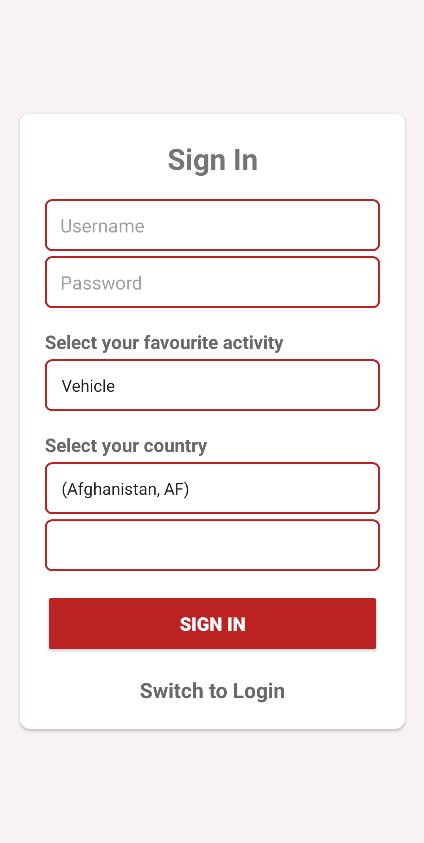
\includegraphics[width=0.35\textwidth]{img1.png}
        }
        \subfigure[Sign In fragment]{
            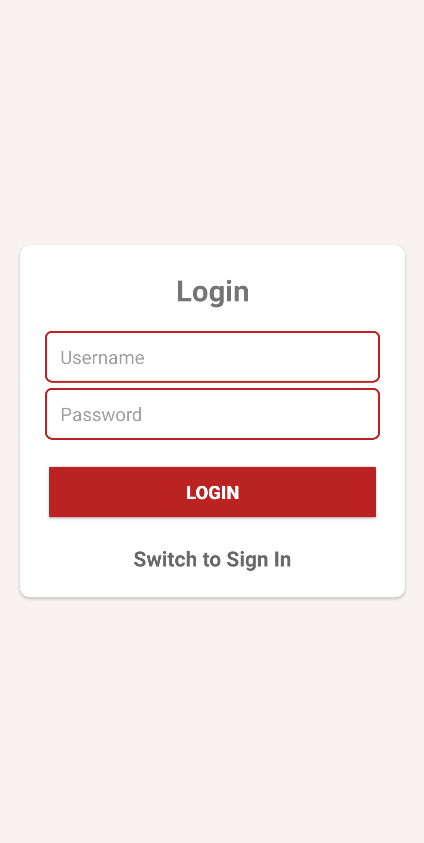
\includegraphics[width=0.35\textwidth]{img2.png}
        }
    \end{figure}
\end{center}
\textit{Registrazione attività} \vspace*{7pt}\\
Proseguendo, successivamente all'autenticazione, è possibile registrare le attività compiute durante la giornata cliccando sul \textit{floating button} presente nella schermata \textbf{Home}, \textbf{Calendario} e \textbf{Grafici}. L'utente può registrare le seguenti attività:
\begin{itemize}
    \renewcommand{\labelitemi}{-}
    \item \textbf{Attività sedentaria}, in cui è definito il tempo trascorso
    \item \textbf{Camminata}, in cui sono memorizzati i passi fatti e il dislivello percorso durante la registrazione
    \item \textbf{Spostamenti in macchina}, durante i quali viene registrata la distanza percorsa
\end{itemize}
Tutti i dati relativi alle attività dell'utente vengono salvati in un database locale e rielaborati per consentirne la visualizzazione grafica. Per consentire ciò è necessario che l'utente, abbia in precedenza autorizzato il permesso \textbf{Activity recognition}. Quest'ultimo garantisce di identificare propriamente l'avvio oppure l'interruzione di un'attività. \vspace*{7pt}\\
\textit{Nota bene}: nel progetto proposto la funzionalità legata al \textbf{detect} dell'attività in corso non consiste in un'\textbf{operazione in background}.
\begin{center}
    \begin{figure}[h]
        \centering
        \subfigure[Registrazione nuove attività]{
            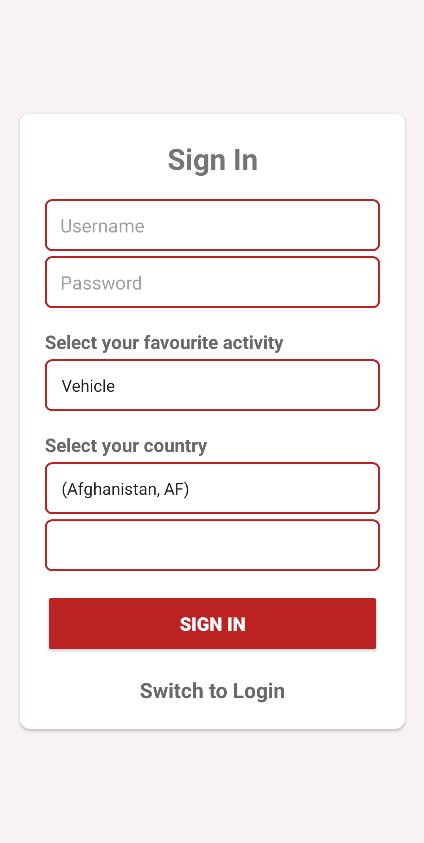
\includegraphics[width=0.35\textwidth]{img1.png}
        }
        \subfigure[Avvio/Interruzione registrazione attività]{
            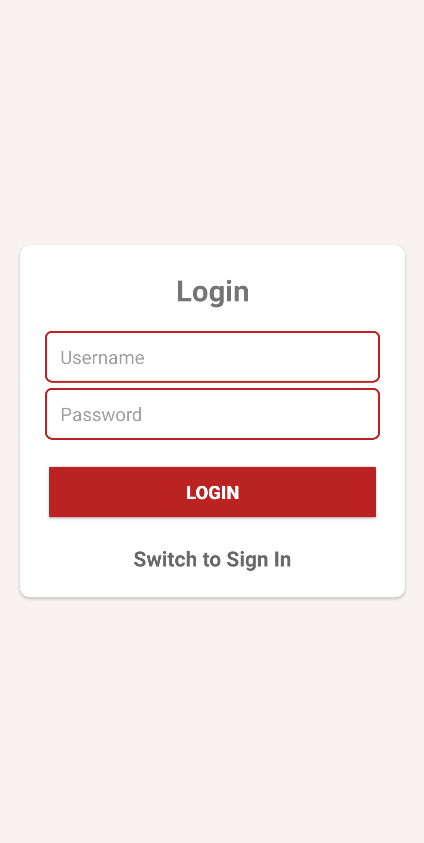
\includegraphics[width=0.35\textwidth]{img2.png}
        }
    \end{figure}
\end{center}
\textit{Calendario} \vspace*{7pt}\\
L'utente può visualizzare nel \textbf{calendario} le attività da lui registrate. Cliccando su una cella del \textit{calendario}, è possibile visualizzare le attività compiute nella giornata selezionata e le relative informazioni, oltre ad un \textit{grafico a torta} che riporta il tempo speso per i vari tipi di attività durante l'arco della giornata, specificando la porzione di tempo di cui non si hanno dati a disposizione.
\begin{center}
    \begin{figure}[h]
        \centering
        \subfigure[Calendario]{
            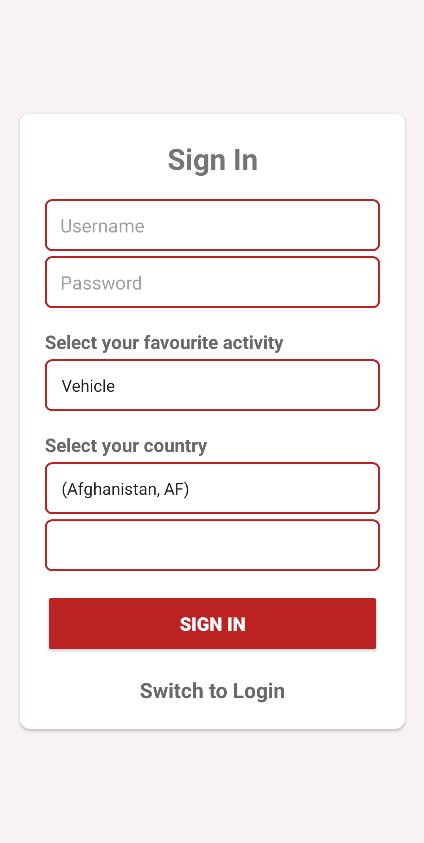
\includegraphics[width=0.35\textwidth]{img1.png}
        }
        \subfigure[Visualizzazione attività]{
            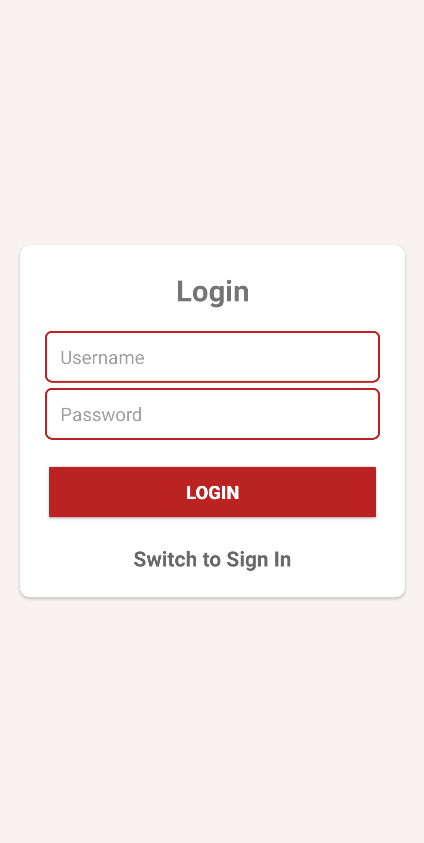
\includegraphics[width=0.35\textwidth]{img2.png}
        }
    \end{figure}
\end{center}
\textit{Grafici} \vspace*{7pt}\\
La feature \textit{grafici} permette di visualizzare in maniera intuitiva i dati registrati dall'applicazione nel mese selezionato. La \textit{View} è composta da tre grafici, cosi suddivisi:
\begin{itemize}
    \renewcommand{\labelitemi}{-}
    \item \textbf{Grafico a barre}, contenente i \textbf{passi fatti} dall'utente ogni giorno registrati durante attività di \textit{camminata}
    \item \textbf{Grafico a barre}, utilizzato per visualizzare la \textbf{distanza percorsa} dall'utente ogni giorno durante le attività di \textit{spostamento con veicolo}
    \item \textbf{Grafico a torta}, che riporta in percentuale la suddivisione per \textbf{tipo di attività} registrate dall'utente
\end{itemize}
\textit{Mappa} \vspace*{7pt}\\
La \textit{View} contiene una \textbf{mappa} all'interno di un \textit{FragmentContainerView}. L'utente può inserire, visualizzare ed eliminare le \textit{aree geografiche di interesse}, registrate all'interno del \textit{database locale}. Una zona di interesse è l'area compresa nel raggio di [150m, 250m] rispetto alle coordinate geografiche selezionate, varcata la soglia di una di esse l'utente riceve una notifica. \vspace*{7pt}\\
\textit{Nota bene}: il funzionamento della feature è garantito solamente in presenza di una connessione dati stabile.
\begin{center}
    \begin{figure}[h]
        \centering
        \subfigure[Mappa]{
            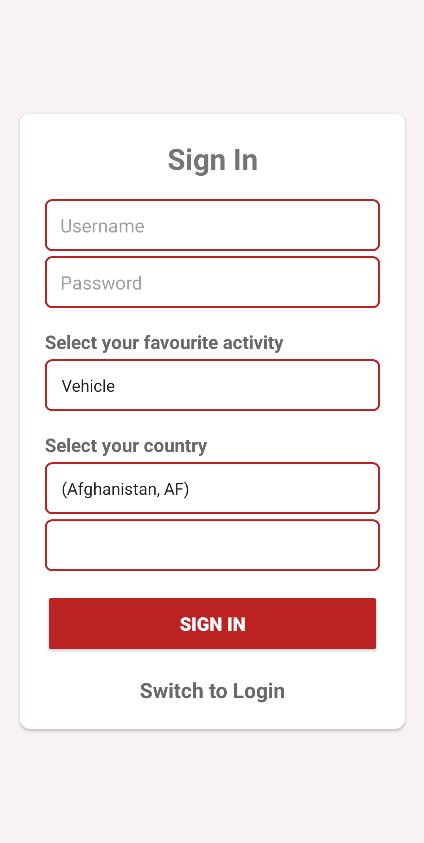
\includegraphics[width=0.35\textwidth]{img1.png}
        }
        \subfigure[Dialog dei marker sulla mappa]{
            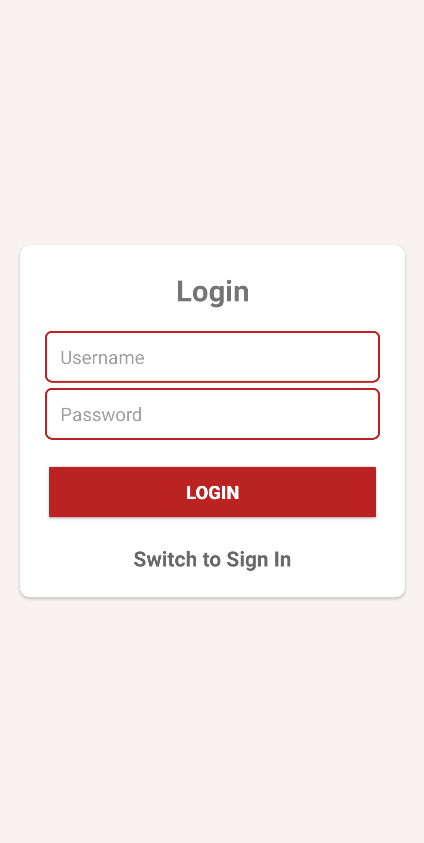
\includegraphics[width=0.35\textwidth]{img2.png}
        }
    \end{figure}
\end{center}
\textit{Amici} \\
Tramite l'applicativo è possibile condividere le proprie attività con gli \textbf{amici} e visualizzare le attività da loro compiute. Un utente può cercare lo \textit{username} di un amico per poi aggiungerlo alle proprie amicizie e visualizzare le attività da esso compiute.
Precedentemente alla condivisione dei dati, all'utente viene mostrato un \textit{Alert Dialog} che richiede l'autorizzazione per il salvataggio dei dati in cloud, se il permesso viene negato sarà comunque possibile visualizzare i dati degli amici.
L'utente può sincronizzare i dati salvati in \textit{cloud} in qualsiasi momento, cliccando sul \textit{floating button} presente nella schermata. \vspace*{7pt}\\
\textit{Nota bene}: il funzionamento della feature è garantito solamente in presenza di una connessione dati stabile.
\newpage
\begin{figure}[h]
    \centering
    \subfigure[Amici fragment]{
        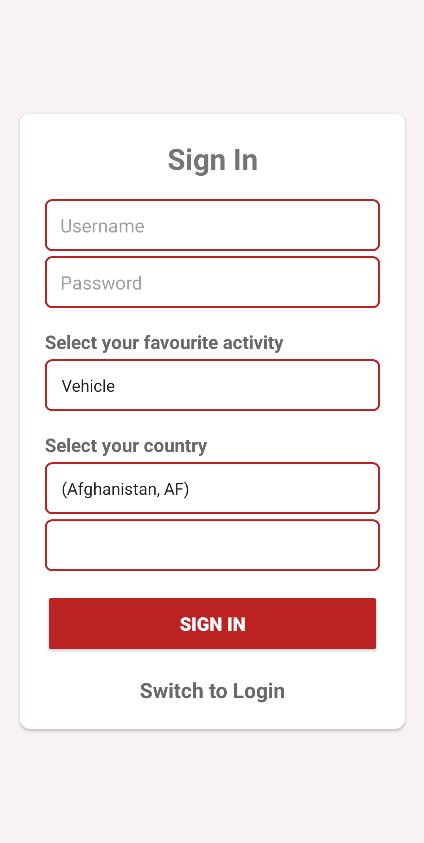
\includegraphics[width=0.35\textwidth]{img1.png}
    }
    \subfigure[Visualizzazione dati amico]{
        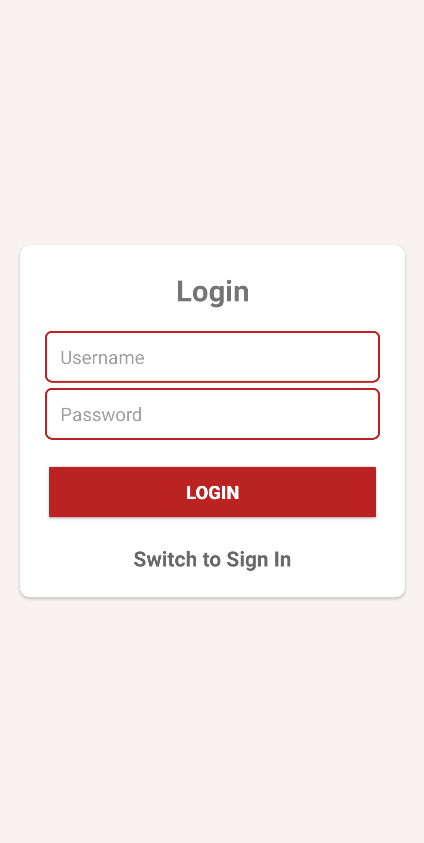
\includegraphics[width=0.35\textwidth]{img2.png}
    }
\end{figure}

\newpage
\subsection*{Scelte implementative}
\subsubsection*{ViewModel}
\subsubsection*{Room}
\subsubsection*{Background operations}
\textit{Geofecing} \\
Receiver - Service - Worker \\
\textit{Connectivity} \\
\subsubsection*{Aws}

\subsection*{Possibili sviluppi futuri}

\end{document}